% ==========================================
% ФАЙЛ: p8.tex
% БЛОК БИЛЕТОВ 36-40 (Сходимость числовых рядов)
% ==========================================

% --- Вопрос 36 ---
\examquestion{36}{Условная сходимость и знакочередующийся гармонический ряд}
{Дайте определение условной сходимости. На примере знакочередующегося гармонического ряда $\sum_{n=1}^{\infty}\frac{(-1)^{n-1}}{n}$ докажите факт его условной сходимости (докажите расходимость ряда из модулей и сходимость самого ряда).}

\paragraph{Суть на пальцах}
Бывают ряды, которые сходятся «из последних сил» только благодаря тому, что их положительные и отрицательные члены взаимно гасят друг друга. Если эту магию отменить и сделать все члены положительными (навесить модуль), ряд тут же «взрывается» и улетает в бесконечность. Такая хрупкая сходимость и называется \textbf{условной}.

\paragraph{1. Определение}
Числовой ряд $\sum_{n=1}^{\infty} a_n$ называется \textbf{условно сходящимся}, если сам ряд сходится, но ряд, составленный из модулей его членов $\sum_{n=1}^{\infty} |a_n|$, расходится.

\paragraph{2. Разбор классического примера}
Исследуем знакочередующийся гармонический ряд:
$$ \sum_{n=1}^{\infty} \frac{(-1)^{n-1}}{n} = 1 - \frac{1}{2} + \frac{1}{3} - \frac{1}{4} + \dots $$

\textbf{Шаг А: Расходимость ряда из модулей}
Составим ряд из абсолютных величин членов:
$$ \sum_{n=1}^{\infty} \left| \frac{(-1)^{n-1}}{n} \right| = \sum_{n=1}^{\infty} \frac{1}{n} = 1 + \frac{1}{2} + \frac{1}{3} + \dots $$
Мы получили классический гармонический ряд. Как известно (из интегрального признака Коши или группировки Орема), он расходится, так как является эталонным рядом Дирихле $\sum \frac{1}{n^p}$ при $p=1 \le 1$. Следовательно, абсолютной сходимости нет.

\textbf{Шаг Б: Сходимость исходного ряда}
Проверим исходный ряд по признаку Лейбница (работает только для Знакочередующихся!!! и смотрим на модули). Проверим два условия:
\begin{enumerate}
    \item Модули членов убывают: $c_n = \frac{1}{n}$. Очевидно, что $c_{n+1} < c_n$ (т.к. $\frac{1}{n+1} < \frac{1}{n}$).
    \item Предел общего члена равен нулю: $\lim_{n \to \infty} \frac{1}{n} = 0$.
\end{enumerate}
Оба условия Лейбница выполнены идеально, значит, исходный ряд сходится.

\textbf{Вывод:} Так как сам ряд сходится, а ряд из его модулей расходится, знакочередующийся гармонический ряд сходится \textbf{условно}.
% --- Вопрос 36 ---
\begin{tcolorbox}[colback=gray!5, colframe=black, boxrule=0.5pt, arc=0pt]
\textbf{Резюмируем Вопрос 36 (Условная сходимость):} \\
\textbf{Тезис:} Ряд сходится «из последних сил», но ряд из модулей расходится (классический пример — знакочередующийся гармонический ряд $\sum \frac{(-1)^{n-1}}{n}$). \\
\textbf{Ход:} Составляем ряд из абсолютных величин членов $\sum \frac{1}{n}$. Он расходится как эталонный ряд Дирихле при $p = 1 \le 1$ (абсолютной сходимости нет). \\
\textbf{Трюк:} Проверяем исходный ряд по признаку Лейбница: модули монотонно убывают ($\frac{1}{n+1} < \frac{1}{n}$), а предел общего члена равен нулю ($\lim \frac{1}{n} = 0$). \\
\textbf{Финал:} Модули расходятся, но сам ряд сходится по Лейбницу $\implies$ сходимость является условной.
\end{tcolorbox}




% --- Вопрос 37 ---
\examquestion{37}{Признак Лейбница и оценка остатка ряда}
{Сформулируйте и докажите теорему Лейбница для рядов вида $\sum(-1)^{n-1}c_{n}$. Докажите монотонность и ограниченность подпоследовательностей четных и нечетных частичных сумм. Приведите геометрическую интерпретацию. Выведите формулу оценки погрешности.}

\paragraph{Суть на пальцах (Геометрия Лейбница)}
Представь кузнечика на числовой прямой, который прыгает вправо, потом влево, потом вправо... Каждый его прыжок короче предыдущего, и в итоге длина прыжка стремится к нулю. Очевидно, что кузнечик не может ускакать в бесконечность — его будет зажимать во всё сужающийся коридор, и он обязательно «приземлится» в одну конкретную точку $S$. При этом его реальное положение всегда находится где-то между точкой после прыжка вправо и точкой после прыжка влево.

\vspace{0.5em}
\begin{center}
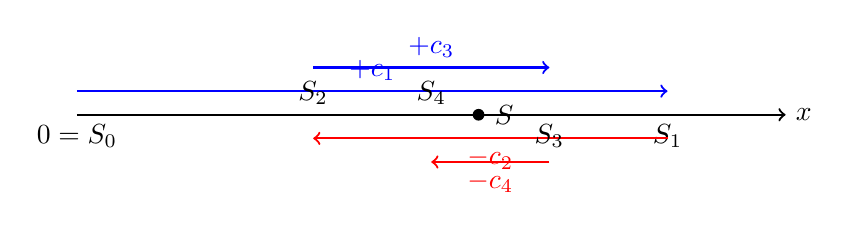
\begin{tikzpicture}[scale=1.5]
    \draw[->, thick] (0, 0) -- (6, 0) node[right] {$x$};
    \node[below] at (0, 0) {$0 = S_0$};
    
    % Прыжки
    \draw[->, blue, thick] (0, 0.2) -- (5, 0.2) node[midway, above] {$+c_1$};
    \node[below] at (5, 0) {$S_1$};
    
    \draw[->, red, thick] (5, -0.2) -- (2, -0.2) node[midway, below] {$-c_2$};
    \node[above] at (2, 0) {$S_2$};
    
    \draw[->, blue, thick] (2, 0.4) -- (4, 0.4) node[midway, above] {$+c_3$};
    \node[below] at (4, 0) {$S_3$};
    
    \draw[->, red, thick] (4, -0.4) -- (3, -0.4) node[midway, below] {$-c_4$};
    \node[above] at (3, 0) {$S_4$};
    
    \node[circle, fill=black, inner sep=1.5pt, label=right:{$S$}] at (3.4, 0) {};
\end{tikzpicture}
\end{center}
\vspace{0.5em}

\paragraph{1. Формулировка теоремы}
Знакочередующийся ряд $\sum_{n=1}^{\infty} (-1)^{n-1} c_n$ (где $c_n \ge 0$) сходится, если выполнены два условия:
1. $c_n \ge c_{n+1}$ (последовательность убывает).
2. $\lim_{n \to \infty} c_n = 0$.

\paragraph{2. Доказательство (через частичные суммы)}
\begin{proof}
Рассмотрим подпоследовательность чётных частичных сумм $S_{2k}$:
$$ S_{2k} = (c_1 - c_2) + (c_3 - c_4) + \dots + (c_{2k-1} - c_{2k}) $$
Так как $c_n \ge c_{n+1}$, каждая скобка $\ge 0$. Значит, при добавлении новой скобки сумма растет: $S_{2k}$ — \textbf{монотонно возрастает}.
С другой стороны, перегруппируем эту же сумму иначе:
$$ S_{2k} = c_1 - (c_2 - c_3) - (c_4 - c_5) - \dots - c_{2k} $$
Здесь из $c_1$ вычитаются неотрицательные скобки. Значит, $S_{2k} \le c_1$, то есть последовательность \textbf{ограничена сверху}.
По теореме Вейерштрасса, монотонная и ограниченная последовательность имеет предел: $\lim_{k \to \infty} S_{2k} = S$.

Теперь рассмотрим подпоследовательность нечётных сумм $S_{2k+1}$:
$$ S_{2k+1} = S_{2k} + c_{2k+1} $$
Перейдем к пределу при $k \to \infty$. Так как по условию $\lim c_{2k+1} = 0$, получаем:
$$ \lim_{k \to \infty} S_{2k+1} = \lim_{k \to \infty} S_{2k} + 0 = S $$
Так как и чётные, и нечётные частичные суммы стремятся к одному числу $S$, то и вся последовательность сумм $S_N$ сходится к $S$. Ряд сходится.
\end{proof}

\paragraph{3. Оценка остатка ряда}
Остаток ряда $R_N$ после отбрасывания $N$ членов сам является рядом Лейбница, который начинается с члена $(-1)^N c_{N+1}$.
По доказанному выше, сумма такого ряда всегда имеет знак своего первого члена и по модулю не превосходит его (ведь из него вычитаются положительные куски).
Следовательно, погрешность ограничена первым отброшенным членом:
$$ |R_N| = |S - S_N| \le c_{N+1} $$

% --- Вопрос 37 ---
\begin{tcolorbox}[colback=gray!5, colframe=black, boxrule=0.5pt, arc=0pt]
\textbf{Резюмируем Вопрос 37 (Признак Лейбница):} \\
\textbf{Тезис:} Знакочередующийся ряд $\sum (-1)^{n-1} c_n$ сходится, если $c_n \searrow 0$. Оценка погрешности: $|R_N| \le c_{N+1}$. \\
\textbf{Ход:} Подпоследовательность чётных частичных сумм $S_{2k}$ монотонно возрастает и ограничена сверху первым членом $c_1$, следовательно, имеет предел $S$ по Вейерштрассу. \\
\textbf{Трюк:} Нечётные суммы выражаем как $S_{2k+1} = S_{2k} + c_{2k+1}$. При $k \to \infty$ добавка $c_{2k+1} \to 0$, поэтому они стремятся к тому же пределу $S$. \\
\textbf{Финал:} Кузнечик зажат в сужающемся коридоре, а остаток ряда по модулю не превышает первого отброшенного слагаемого.
\end{tcolorbox}




% --- Вопрос 38 ---
\examquestion{38}{Преобразование Абеля (Суммирование по частям)}
{Сформулируйте и докажите лемму о преобразовании Абеля для конечных последовательностей $\{a_{k}\}$ и $\{b_{k}\}$. Введя обозначение для частичных сумм $B_{k}=\sum_{j=1}^{k}b_{j}$ (положив $B_{0}=0$), проведите вывод тождества.}

\paragraph{Суть на пальцах}
Преобразование Абеля — это \textbf{дискретный аналог интегрирования по частям} ($\int u\,dv = uv - \int v\,du$). Вместо интегралов у нас суммы ($\Sigma$), а вместо дифференциалов — конечные разности ($\Delta a_k = a_k - a_{k+1}$). Мы «перекидываем» операцию суммирования с одной последовательности ($b_k$) на другую ($a_k$), что невероятно полезно, когда $b_k$ ведет себя хаотично, но имеет ограниченные суммы, а $a_k$ гладко убывает.

\paragraph{1. Формулировка леммы}
Для любых конечных последовательностей $\{a_k\}_{k=1}^n$ и $\{b_k\}_{k=1}^n$ справедливо тождество (дискретная формула суммирования по частям):
$$ \sum_{k=1}^n a_k b_k = a_n B_n + \sum_{k=1}^{n-1} (a_k - a_{k+1}) B_k $$
где $B_k = b_1 + b_2 + \dots + b_k$ — частичные суммы (при этом $B_0 = 0$).

\paragraph{2. Вывод тождества (Доказательство)}
\begin{proof}
Выразим элементы последовательности $b_k$ через частичные суммы:
$$ b_k = B_k - B_{k-1} \quad \text{(это верно даже для } k=1 \text{, так как } B_0 = 0\text{)} $$
Подставим это выражение в исходную сумму:
$$ \sum_{k=1}^n a_k b_k = \sum_{k=1}^n a_k (B_k - B_{k-1}) = \sum_{k=1}^n a_k B_k - \sum_{k=1}^n a_k B_{k-1} $$
Во второй сумме сделаем сдвиг индекса суммирования (заменим $k$ на $k+1$):
$$ \sum_{k=1}^n a_k b_k = \sum_{k=1}^n a_k B_k - \sum_{k=0}^{n-1} a_{k+1} B_k $$
Выделим "граничные" члены, которые не попадают в общую область индексов от $1$ до $n-1$:
\begin{itemize}
    \item Из первой суммы отщепляем последнее слагаемое (при $k=n$): $a_n B_n$.
    \item Из второй суммы отщепляем первое слагаемое (при $k=0$): $a_1 B_0$.
\end{itemize}
Тогда оставшиеся части можно объединить под один знак суммы:
$$ \sum_{k=1}^n a_k b_k = a_n B_n - a_1 B_0 + \sum_{k=1}^{n-1} a_k B_k - \sum_{k=1}^{n-1} a_{k+1} B_k $$
Вынесем $B_k$ за скобки. Учтем, что $B_0 = 0$ по определению, поэтому слагаемое $a_1 B_0$ исчезает:
$$ \sum_{k=1}^n a_k b_k = a_n B_n + \sum_{k=1}^{n-1} (a_k - a_{k+1}) B_k $$
Тождество полностью доказано.
\end{proof}


% --- Вопрос 38 ---
\begin{tcolorbox}[colback=gray!5, colframe=black, boxrule=0.5pt, arc=0pt]
\textbf{Резюмируем Вопрос 38 (Преобразование Абеля):} \\
\textbf{Тезис:} Дискретный аналог интегрирования по частям: $\sum_{k=1}^n a_k b_k = a_n B_n + \sum_{k=1}^{n-1} (a_k - a_{k+1}) B_k$, где $B_k = \sum_{j=1}^k b_j$. \\
\textbf{Ход:} Выражаем элементы через частичные суммы $b_k = B_k - B_{k-1}$ (полагая $B_0 = 0$) и подставляем в исходную сумму. \\
\textbf{Трюк:} Раскрываем скобки и сдвигаем индекс суммирования во второй части, чтобы сгруппировать слагаемые с общим множителем $B_k$. \\
\textbf{Финал:} Отщепляем граничные слагаемые $a_n B_n$ и $a_1 B_0$ (последний обнуляется) и сводим остаток под единую сумму.
\end{tcolorbox}



а теперь перейдем к .....
$\vcenter{\hbox{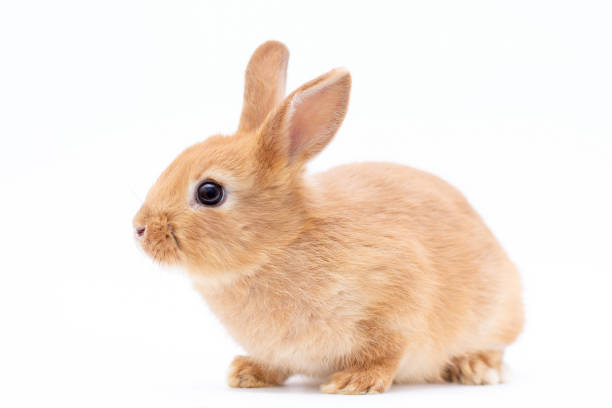
\includegraphics[height=1.2em]{rabbit.png}}}$ \hspace{0.5em} 
{)))}
% --- Вопрос 39 ---
\examquestion{39}{Признак Дирихле сходимости числовых рядов}
{Сформулируйте признак Дирихле. Используя преобразование Абеля и критерий Коши, докажите теорему. На примере $\sum\frac{\sin n}{n^p}$ докажите сходимость при $p>0$ и исследуйте область условной сходимости.}

\paragraph{Суть на пальцах}
$\vcenter{\hbox{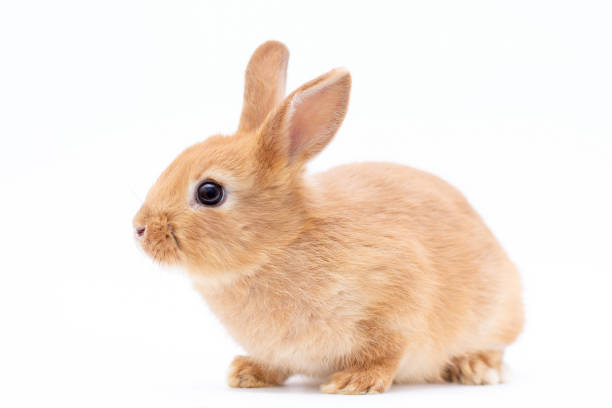
\includegraphics[height=1.2em]{rabbit.png}}}$ \hspace{0.3em}
Признак Дирихле работает с рядом $\sum a_n b_n$. Представь, что $b_n$ — это пружина: она болтается туда-сюда, но её размах ограничен стенками (частичные суммы ограничены). А $a_n$ — это амортизатор: он плавно и без рывков гасит всё в ноль ($a_n \searrow 0$). Амортизатор неизбежно задушит пружину, и ряд сойдется.

\paragraph{1. Формулировка теоремы}
Ряд $\sum_{n=1}^{\infty} a_n b_n$ сходится, если выполнены два условия:
\begin{enumerate}
    \item \textbf{Суммы $b_n$ ограничены:} $\exists M > 0$, такое что $\forall N$ выполняется $|B_N| = \left| \sum_{k=1}^N b_k \right| \le M$.
    \item \textbf{$a_n$ монотонно убывает к нулю:} $a_n \searrow 0$ при $n \to \infty$.
\end{enumerate}

\paragraph{2. Доказательство теоремы}
\begin{proof}
Будем доказывать сходимость ряда, используя \textbf{критерий Коши}: нам нужно показать, что для любого $\varepsilon > 0$ найдется номер $N$, такой что $\forall n > N$ и $\forall p \ge 1$ выполняется неравенство $\left| \sum_{k=n+1}^{n+p} a_k b_k \right| < \varepsilon$.

Рассмотрим кусок ряда и применим \textbf{преобразование Абеля}. Выразим $b_k = B_k - B_{k-1}$ (считая $B_0 = 0$):
$$ \sum_{k=n+1}^{n+p} a_k b_k = \sum_{k=n+1}^{n+p} a_k (B_k - B_{k-1}) $$

Раскроем скобки и перегруппируем слагаемые при одинаковых $B_k$:
$$ \sum_{k=n+1}^{n+p} a_k b_k = -a_{n+1} B_n + a_{n+p} B_{n+p} + \sum_{k=n+1}^{n+p-1} B_k (a_k - a_{k+1}) $$

Берем всё выражение по модулю и применяем неравенство треугольника:
$$ \left| \sum_{k=n+1}^{n+p} a_k b_k \right| \le |-a_{n+1} B_n| + |a_{n+p} B_{n+p}| + \sum_{k=n+1}^{n+p-1} |B_k| \cdot |a_k - a_{k+1}| $$

По первому условию все $|B_k| \le M$. Заменяем модули сумм на $M$ и выносим за скобки:
$$ \left| \sum_{k=n+1}^{n+p} a_k b_k \right| \le M a_{n+1} + M a_{n+p} + M \sum_{k=n+1}^{n+p-1} |a_k - a_{k+1}| $$

По второму условию $a_k$ монотонно убывает, значит разность $(a_k - a_{k+1}) \ge 0$, и модуль внутри суммы можно просто опустить. Сумма разностей является телескопической и схлопывается по принципу домино:
$$ \sum_{k=n+1}^{n+p-1} (a_k - a_{k+1}) = (a_{n+1} - a_{n+2}) + (a_{n+2} - a_{n+3}) + \dots + (a_{n+p-1} - a_{n+p}) = a_{n+1} - a_{n+p} $$

Подставляем этот результат обратно в наше неравенство:
$$ \left| \sum_{k=n+1}^{n+p} a_k b_k \right| \le M a_{n+1} + M a_{n+p} + M (a_{n+1} - a_{n+p}) = 2M a_{n+1} $$

Так как $\lim_{n \to \infty} a_n = 0$, то при достаточно больших $n$ выражение $2M a_{n+1}$ станет строго меньше $\varepsilon$. Критерий Коши выполнен $\implies$ ряд сходится.
\end{proof}

\paragraph{3. Эталонный разбор: ряд $\sum_{n=1}^{\infty} \frac{\sin n}{n^p}$}
Здесь $a_n = \frac{1}{n^p}$, а $b_n = \sin n$.

\textbf{Шаг 1: Ограниченность $\sum \sin n$}
Запишем частичную сумму $B_N = \sum_{k=1}^N \sin k$. Умножим и разделим её на константу $2\sin(1/2)$:
$$ B_N = \frac{\sum_{k=1}^N 2\sin k \cdot \sin(1/2)}{2\sin(1/2)} $$
По школьной формуле $2\sin\alpha\sin\beta = \cos(\alpha-\beta) - \cos(\alpha+\beta)$ числитель превращается в цепь сокращающихся косинусов:
$$ (\cos 0.5 - \cancel{\cos 1.5}) + (\cancel{\cos 1.5} - \cancel{\cos 2.5}) + \dots - \cos(N+0.5) = \cos 0.5 - \cos(N+0.5) $$
Оцениваем модуль дроби (косинусы не превышают 1):
$$ |B_N| \le \frac{1 + 1}{2\sin(1/2)} = \frac{1}{\sin(1/2)} = M $$
Суммы $b_n$ ограничены константой $M$. Условие 1 выполнено.

\textbf{Шаг 2: Анализ по параметру $p$}
\begin{itemize}
    \item \textbf{При $p > 0$:} $a_n = \frac{1}{n^p}$ монотонно стремится к нулю. Условие 2 выполнено. \textbf{Ряд сходится.}
    \item \textbf{При $p > 1$ (Абсолютная сходимость):} $\left|\frac{\sin n}{n^p}\right| \le \frac{1}{n^p}$. Так как ряд $\sum \frac{1}{n^p}$ сходится при $p>1$, то и наш ряд сходится \textbf{абсолютно}.
    \item \textbf{При $0 < p \le 1$ (Условная сходимость):} Проверим ряд из модулей. Используем формулу $|\sin n| \ge \sin^2 n = \frac{1 - \cos 2n}{2}$:
    $$ \sum \frac{|\sin n|}{n^p} \ge \frac{1}{2}\sum \frac{1}{n^p} - \frac{1}{2}\sum \frac{\cos 2n}{n^p} $$
    Ряд с косинусом сходится (по тому же Дирихле), а ряд $\sum \frac{1}{n^p}$ при $p \le 1$ \textbf{расходится}. Значит, ряд модулей расходится. Сходимость \textbf{только условная}.
\end{itemize}



% --- Вопрос 39 ---
\begin{tcolorbox}[colback=gray!5, colframe=black, boxrule=0.5pt, arc=0pt]
\textbf{Резюмируем Вопрос 39 (Признак Дирихле):} \\
\textbf{Тезис:} Ряд $\sum a_n b_n$ сходится, если частичные суммы $B_N$ ограничены константой $M$, а $a_n$ монотонно стремится к нулю. \\
\textbf{Ход:} Применяем к «хвосту» ряда критерий Коши и преобразование Абеля, заменяя суммы $B_k$ на их верхнюю границу $M$. \\
\textbf{Трюк:} Оставшаяся разность $(a_k - a_{k+1})$ образует телескопическую сумму, которая схлопывается в простую разность $a_{n+1} - a_{n+p}$. \\
\textbf{Финал:} Оценка сводится к выражению $2M a_{n+1}$, стремящемуся к нулю (работает, например, для исследования условной сходимости $\sum \frac{\sin n}{n^p}$ при $p > 0$).
\end{tcolorbox}






% --- Вопрос 40 ---
\examquestion{40}{Признак Абеля сходимости числовых рядов}
{Сформулируйте и докажите признак Абеля (сводя к признаку Дирихле с помощью метода центрирования). Обоснуйте, почему требование сходимости базового ряда позволяет ослабить требования к $a_n$.}

\paragraph{Суть на пальцах}
Признак Абеля — это брат признака Дирихле, но силы распределены иначе. Теперь ряд $b_n$ сам по себе \textbf{хороший и сходящийся} (ему не нужно помогать сходиться). А функция $a_n$ просто не должна всё испортить. Поэтому к $a_n$ требование ослаблено: ей \textit{не обязательно} затухать до нуля, достаточно просто не «раскачивать лодку» — то есть быть монотонной и ограниченной. 

\paragraph{1. Формулировка теоремы}
Ряд $\sum_{n=1}^{\infty} a_n b_n$ сходится, если выполнены два условия:
1. Ряд $\sum_{n=1}^{\infty} b_n$ \textbf{сходится}.
2. Последовательность $a_n$ \textbf{монотонна и ограничена}.

\paragraph{2. Доказательство (метод центрирования монотонного сомножителя)}
\begin{proof}
Так как последовательность $a_n$ монотонна и ограничена, по теореме Вейерштрасса она имеет конечный предел. Пусть $\lim_{n \to \infty} a_n = A$.
Центрируем последовательность, введя новую переменную $\alpha_n = a_n - A$. 
Очевидно, что $\alpha_n$ монотонна (так как $a_n$ монотонна) и стремится к нулю ($\lim \alpha_n = A - A = 0$).

Перепишем общий член нашего ряда через новую переменную:
$$ a_n b_n = (A + \alpha_n)b_n = A \cdot b_n + \alpha_n b_n $$
Рассмотрим сумму этого ряда как сумму двух независимых рядов:
$$ \sum_{n=1}^{\infty} a_n b_n = \sum_{n=1}^{\infty} A \cdot b_n + \sum_{n=1}^{\infty} \alpha_n b_n $$

Исследуем каждый кусок:
\begin{enumerate}
    \item Ряд $\sum A \cdot b_n = A \sum b_n$. Так как исходный базовый ряд $\sum b_n$ сходится по условию, то и умноженный на константу $A$ он тоже сходится.
    \item Ряд $\sum \alpha_n b_n$. Применим к нему признак Дирихле:
    \begin{itemize}
        \item Частичные суммы $B_n$ ограничены (и даже более того — они имеют конечный предел, так как $\sum b_n$ сходится).
        \item $\alpha_n$ монотонно стремится к нулю (мы так её сконструировали).
    \end{itemize}
    Значит, по признаку Дирихле (Вопрос 39) второй ряд сходится.
\end{enumerate}
Так как исходный ряд $\sum a_n b_n$ представлен суммой двух сходящихся рядов, он сам гарантированно сходится.
\end{proof}

\paragraph{3. Обоснование ослабления требований}
В признаке Дирихле базовый ряд $\sum b_n$ не сходился (например, просто болтался $+1, -1, +1, -1$). Чтобы «принудительно» заставить его сойтись, нам требовался жесткий амортизатор $a_n \to 0$.
В признаке Абеля базовый ряд $\sum b_n$ \textbf{уже сошелся сам}. Нам не нужно тянуть его к нулю. Нам нужно только гарантировать, что домножение на $a_n$ не вызовет резонанс. Условие «монотонность + ограниченность» как раз и означает, что $a_n$ просто плавно масштабирует члены $b_n$, не разрушая хрупкую структуру сходимости базового ряда.

% --- Вопрос 40 ---
\begin{tcolorbox}[colback=gray!5, colframe=black, boxrule=0.5pt, arc=0pt]
\textbf{Резюмируем Вопрос 40 (Признак Абеля):} \\
\textbf{Тезис:} Ряд $\sum a_n b_n$ сходится, если базовый ряд $\sum b_n$ уже сходится, а последовательность $a_n$ просто монотонна и ограничена. \\
\textbf{Ход:} По теореме Вейерштрасса у монотонной ограниченной последовательности есть предел $A$. Центрируем её, вводя величину $\alpha_n = a_n - A$, которая стремится к нулю. \\
\textbf{Трюк:} Раскладываем общий член на две составляющие: $A \cdot b_n + \alpha_n b_n$, расщепляя исходный ряд на две суммы. \\
\textbf{Финал:} Первый ряд сходится, так как сходится базовый $\sum b_n$. Второй сходится по признаку Дирихле ($\alpha_n \to 0$ при ограниченных суммах). Жёсткого затухания $a_n$ не требуется, так как $\sum b_n$ не требует дополнительного «гашения».
\end{tcolorbox}